\subsection{Client Subsystem}
The client layer subsystem will display the UI of the application. 
It has a XY graph and a dot calculator.
It has a button for record the voice of the users

\begin{figure}[h!]
	\centering
 	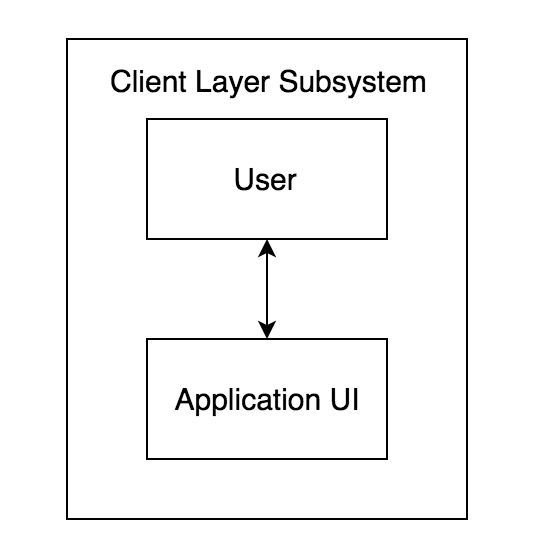
\includegraphics[width=0.60\textwidth]{images/subsystem_client}
 \caption{Client subsystem diagram}
\end{figure}

\subsubsection{Assumptions}
The users press the record button, it will be recorded the sound and display the accurate dot.

\subsubsection{Responsibilities}
The Client Layer Subsystem will send the user's voice to the application, and interaction with user. And it will display a dot on the application UI.
The Client Layer should display all information to user. And receive user's request.

\subsubsection{Subsystem Interfaces}
Each of the inputs and outputs for the subsystem are defined here. Create a table with an entry for each labelled interface that connects to this subsystem. For each entry, describe any incoming and outgoing data elements will pass through this interface.

\begin {table}[H]
\caption {Client Subsystem interfaces} 
\begin{center}
    \begin{tabular}{ | p{1cm} | p{6cm} | p{3cm} | p{3cm} |}
    \hline
    ID & Description & Inputs & Outputs \\ \hline
    \#1 & XY Graph & \pbox{3cm}{N/A} & \pbox{3cm}{Red dot}  \\ \hline
    \#2 & Voice Record Button & \pbox{3cm}{User's sound} & \pbox{3cm}{N/A}  \\ \hline
    \end{tabular}
\end{center}
\end{table}
